\chapter{Learning to Rank}

A ranking algorithm is a function that takes a set of documents and a query, and returns a ranked list of documents. In previous chapters, it was shown how to determine the relevance a document has with regards to a query by converting them into a vector representation of words, and then calculating some similarity score (e.g., cosine similarity). However, this approach does not consider many factors (other than word frequency) that can influence relevance, such as co-occurence of words, or the position of a term in the fields of the document, such as title, abstract, or body; other factors may be the in-degree and out-degree of a webpage, the number of clicks it received, or the anchor text used to refer to the page in external links.

Modern search engines do in fact consider several statistics that are not limited to word frequency. As the size and complexity of documents and queries grow, building a custom function to rank documents becomes more and more difficult: for this reason, the problem of ranking is dealt with as a supervised machine learning task, called \textbf{Learning to Rank} (\textbf{LtR}).

\section{Machine Learning Basics}

\textbf{Machine Learning} is a field of computer science that deals with the study and usage of statistical methods to enable computers to learn from data without being explicitly programmed to do so. After learning, the computer can make predictions, decisions, or generate new data based on the patterns it found in the input data. There exist many \textbf{models} in machine learning, each of which ``learns'' from data differently. 

The input data forms the \textbf{training set}; any data used to test the performance of the model forms the \textbf{test set}. Each item in a dataset is called \textbf{instance} (or example, pattern); each instance is described by a set of \textbf{features} (also called attributes). In a tabular dataset, typically each row is an instance, and each column is a feature.
\\
Machine learning tasks can be categorized into two main groups:
\begin{itemize}
    \item \textbf{Supervised learning}: given a training set of input-ouput pairs $<x_i,y_i>$ for an unknown function $f$ (called \textbf{target function}), such that $f(x_i) = y_i + \epsilon$, the goal is to find a reasonably good approximation of $f$. $\epsilon$ is a random error term, called \textbf{noise}, which cannot be separated from the output. $y_i$ is called \textbf{target value} of $x_i$.
    
    The most well-known supervised learning tasks are \textbf{regression}, in which the function to be approximated is real-valued, and \textbf{classification}, in which the function is discrete-valued and returns a class labeling.

    \item \textbf{Unsupervised Learning}: same as above, but the training set only contains input data $x_i$, and the goal is to find some inherent structure in the data.

    A typical unsupervised learning task is clustering, in which the goal is to find groups of similar data points.
\end{itemize}
Both supervised and unsupervised tasks have a training phase and a testing phase: the first is done offline, while the second is often done online.

The way models are trained is by gradually adapting some initial approximation of the target function, modifying its parameters so that the error between the predicted output and the actual output is minimized over a number of repetitions, called \textbf{epochs}. To measure the error and recalculate the changes to apply to the parameters at each epoch, a \textbf{loss function} is used. The loss function is a measure of how well the model is performing, and may also contain some optional terms to control the updates of the parameters. There exist different loss functions, each suited for different tasks and models. Some common loss functions include Mean Squared Error (MSE):
\begin{equation*}
    \textit{MSE} = \frac{1}{n} \sum_{i=1}^n (y_i - \hat{f}(x_i))^2
\end{equation*}
and Mean Absolute Error (MAE):
\begin{equation*}
    \textit{MAE} = \frac{1}{n} \sum_{i=1}^n |y_i - \hat{f}(x_i)|
\end{equation*}
Here, $\hat{f}$ refers to the model's approximation of the target function.

To train the model, many algorithms have been developed; a common choice is \textbf{gradient descent}, which requires the loss function to be differentiable as it uses the inverse of its gradient as the direction in which it decreases.

\section{Learning to Rank}

In a LtR task, the data is represented by queries, documents, and ranks. As mentioned above, representing documents and queries as vectors of words alone is not enough to best capture relevance. Features in LtR can be divided into three groups: \textbf{query-only}, such as query type and length, \textbf{query-independent}, that exclusively depend on the characteristics of the document such as PageRank or URL length, and \textbf{query-dependent}, that are document characteristics that depend on the query, such as BM25 score, query-URL click count, or query word placement in the document.

For example, assume we are given the following training dataset:
\begin{table}[H]
    \centering
    \begin{tabular}{|c|c||c|c|c|c|}
    \hline
    docID & Query & $\alpha$ & $\omega$ & Judgement \\
    \hline
    37 & amazon rainforest & 0.03 & 2 & 1 \\
    37 & gorilla lifespan & 0.012 & 55 & 0 \\
    49 & big cats africa & 0.06 & 5 & 1 \\
    54 & coral reef & 0.007 & 21 & 0 \\
    105 & paperino free download & 0.0001 & 1046 & 0 \\
    105 & ringed seals sachalin & 0.041 & 4 & 1 \\
    \hline
    \end{tabular} 
\end{table} 
Here, the document ID and the query text are not to be used as input to the model, but are just used to uniquely identify pairs. The actual input data is represented by the cosine similarity ($\alpha$) and the shortest text span ($\omega$), i.e., the number of words between the first and last word of a query in the document (not considering the specific order). The output values are binary relevance judgements, where 1 means relevant, and 0 means not relevant. \\
A simple model to represent the relationship between the input and output features is the linear model:
\begin{equation*}
    \textit{score}(d,q) = \textit{score}(\alpha, \omega) = w_1 \cdot \alpha + w_2 \cdot \omega + b
\end{equation*}
The classifier is trained to find the values of $w_1$, $w_2$, and $b$, such that if $\textit{score}(d,q) > b$, the document is classified as relevant, otherwise it is non-relevant. If we interpret the features of the instances as coordinates in a 2D space, we can interpret the function found by the model as a line (or in general, of an $n$-dimensional hyperplane) that separates the relevant documents from the non-relevant ones.
\begin{figure}[H]
    \centering
    \includesvg[width=0.5\textwidth]{img/linear_model.svg}
    \caption{Graphical representation of a linear model in a 2D space.}
\end{figure}
As it can be seen in the figure, the line does not perfectly separate the two classes, but admits some errors. This is not a bad thing, as real world data is very unlikely to be linearly separable. Even when using models capable of approximating non-linear functions, like neural networks, we still want to prevent them from perfectly separating the classes; in general, we don't want the model to produce no errors on the training data, as this would cause what is known as \textbf{overfitting}. If a model overfits the training data, it will perform poorly on the test data, and any other data it has not seen before.

\paragraph{BM25F}
BM25 is a probabilistic ranking function that assumes terms are independent to estimate the probability of a document being relevant with respect to a query. It considers not only term frequency, but also document length. It can be interpreted as:
\begin{equation*}
    \textit{BM25}(d,q) = \sum_t \textit{idf}_t \tau(F_t)
\end{equation*}
where $F_t$ is the term frequency normalized using the hyperparameter $b$:
\begin{equation*}
    F_t = \frac{f_{t,d}}{1 - b + b \cdot |D|/\textit{avgdl}}
\end{equation*}
and $\tau$ is a \textbf{saturation function} that models non-linearity of the contribution of term frequencies:
\begin{equation*}
    \tau(F_t) = \frac{F_t}{k_1 + F_t}.
\end{equation*}

BM25 can be extended to handle structured documents, such as HTML pages or research papers, that have different fields (e.g., head, title, body, URL, tags, abstract, summary, author). The extended function is called \textbf{BM25F} (``F'' stands for ``field''). The BM25F function is:
\begin{align*}
    &\textit{BM25F}(d,q) = \sum_t \textit{idf}_t \tau(F_t) \ , & F_t = \sum_s \frac{w_s \cdot f_{t,s}}{1 - b_s + b_s \cdot |D_s|/\textit{avgdl}_s}
\end{align*}
where:
\begin{itemize}[noitemsep]
    \item $w_s$ is the weight assigned to field $s$;
    \item $f_{t,s}$ is the frequency of term $t$ in field $s$ of document $d$;
    \item $|D_s|$ is the length of field $s$ of document $d$;
    \item $b_s$ is the normalization parameter for field $s$;
    \item $\textit{avgdl}_s$ is the average length of field $s$ in the collection.
\end{itemize}
$k_1$ does not change, since it does not depend on the fields themselves.

This function has a total of $2s + 1$ free parameters ($s$ is the number of fields). To find the best value to assign to these parameters, we can use a Learning to Rank framework: the training data is a set of queries and corresponding set of results, each annotated with a relevance label/score, and the objective is to learn, among all possible BM25 functions, the one that best reflects the relationship between intput and output features. A key issue, however, is that we evaluate the performance of the model using a measure that is calculated over a ranking, such as NDCG. Since this function is not differentiable, we cannot directly apply common algorithms such as gradient descent to optimize the parameters of the model. Ways to overcome this issue will be shown in the next sections.

\subsection{Learning to Rank Approaches}

Depending on how input data is represented, we can distinguish between three main approaches to LtR:
\begin{itemize}
    \item \textbf{Pointwise}, where each query-document is its own example, and is associated with a score.
    \item \textbf{Pairwise}, where each query is accompanied by two documents, one more relevant than the other for that query.
    \item \textbf{Listwise}, where each query is accompanied by an ideal ranking of documents.
\end{itemize}

\paragraph{Pointwise Approach}
With pointwise methods, the idea is to reduce the problem to a simple classification,  regression, or ordinal regression task. The model is trained to predict the degree of relevance of each document with respect to a given query, independently of others. Obviously, since there is no actual ranking to be learned or predicted, this approach is not sufficient for most applications.

\paragraph{Pairwise Approach}
Pairwise methods models the target function as a function of a query and a pair of documents, returning a score that indicates how much more relevant one document is compared to the other. The error can then be calculated as how correctly the ideal ordering of any two pair of documents is predicted.

An example of pairwise method is \textbf{RankNet}. Given two documents, $d_i$ and $d_j$, it models the probability that $d_i$ is more relevant than $d_j$ using the logistic function:
\begin{equation*}
    P_{ij} = \frac{e^{o_{ij}}}{1 + e^{o_{ij}}} = \frac{1}{1 + e^{-o_{ij}}}
\end{equation*}
where $o_{ij}$ is the difference between the outputs assigned to $d_i$ and $d_j$. As a loss function, it uses the cross-entropy loss:
\begin{equation*}
    C_{ij} = - T_{ij} \log P_{ij} - (1 - T_{ij}) \log (1 - P_{ij})
\end{equation*}
where $T_{ij}$ is the score found in the training data for that pair, either 1 if $d_i$ is more relevant than $d_j$, or 0 otherwise. Since this loss is differentiable, the model can be trained using gradient descent.

\paragraph{Listwise Approach}
Listwise approaches include a large family of models. \textbf{LambdaMART} extends the RankNet objective by using a heuristic, where the contribution to the error of pair of documents is either reduced or amplified by a multiplicative factor that correlates with the change in NDCG if the two documents were to be swapped in the ranking. In practice, this is a boosted tree model where the output is calculated as the combined output of several small, weak regression trees.

Deep neural networks are another powerful machine learning model that can be used for LtR. They can be combined with other models: for example, the neural network can be trained on the output produced by LambdaMart, rather than the training labels, enriching the dataset with points around discontinuities in the input space.

\subsection{Pipelined Ranking}
Once we have (efficiently) trained a model to solve our LtR task, that found a function with minimal complexity required to approximate the target function, we must apply it to the user queries as they are received by the system. Since this is done online, efficiency is crucial. A naive approach is \textbf{single-stage ranking}: we use the trained model, give it as input a user query and the set of matching documents, and produce a ranking. However, the set of matching documents may be too large for the model to proecess them efficiently, since for each of them it must translate them into feature vectors (which means calculating cosine similarity, BM25, etc., for each query-document pair), and then apply the model to the input, which may be computationally expensive in itself.

To improve the process, we can consider three efficiency vs. effectiveness trade-offs:
\begin{itemize}
    \item \textbf{Feature computation}: we either have computationally expensive but highly discriminative features, or computationally cheap but only slightly discriminative features. 
 
    \item \textbf{Number of matching candidates}: we either consider a large set of candidates, which is expensive but produces a higher-quality result, or we consider a small set of candidates, which is faster, but may produce low-quality results. 

    \item \textbf{Model complexity}: we either build a complex, slow, and high quality model, or a simple, fast, but low quality model.
\end{itemize}

To handle these trade-offs, we can use a \textbf{two-stage ranking} or, in general, \textbf{multi-stage ranking} pipeline, where multiple rankers are combined to produce a result. A common strategy for two-stage pipelining is to use a recall-oriented ranker to isolate a subset of $k$ documents, which are then used as input for a precision-oriented ranker. The first ranker is trained to maximize the number of relevant documents in the top $k$ positions, while the second ranker is trained to maximize the quality of the ranking in the top $k$ positions. In multi-stage ranking, multiple rankers can be used, each with a different objective. This also allows the pipeline to control which features are used when evaluating the documents, as well as control the complexity of each step.

\section{Gradient Boosting Machines}

\textbf{Ensemble methods} consist in training multiple weak models and combining their outputs to produce a single answer; even though the individual models are not very accurate by themselves, the aggregation of their answer can produce a good result. The biggest advantage of ensemble models is that there is no unique model to train, which may take a lot of time and resources, but rather many simple models that can be trained quickly and sometimes in parallel. In general, when the task to be solved is of classification, the final output is the majority vote of the models, while for regression tasks, the output is the mean of the models' outputs. Depending on the specific method used, the majority vote or the mean can be weighted so that certain models have more influence than others.

\textbf{Gradient boosting machines} are a type of ensemble model that uses decision trees as its base models. A \textbf{decision tree} is a machine learning model that gradually splits the input space into smaller and smaller regions as the training goes on, so that each region can be associated with a single output: the most represented class if it's a classification task, or the mean of the target values if it's a regression task. Each region of the input space can be represented by a node in a tree, and each split is represented by outgoing edges that produce new nodes (new regions). The nodes at the end of the tree, i.e., the leaves, contain the final output.

The splits are done by choosing a feature, and a specific value for it to use as a threshold. If the feature is continuous, the input instances are split between those that have a value greater than the threshold, and those that have a value less than the threshold. If the feature is discrete, the instances are split between those that have the same value as the treshold, and those that don't. This process is repeated until some stopping condition is valid; common choices are tree depth, leaf purity, or number of leaves.

In a gradient boosting machine, a set of small decision trees is trained in sequence, so that each tree tries to correct the errors made by the previous one. Each tree contributes to a partial score: to calculate the final output, all the partial scores of all trees are summed together. Each decision tree must be relatively small (in terms of both depth and total number of nodes).

\begin{figure}[H]
    \centering
    \includesvg[width=0.8\textwidth]{img/dectree.svg}
    \caption{Example of a decision tree.}
\end{figure} 

Let's now formalize the gradient boosting algorithm: given the input data $<x_i,y_i>$, where each $x_i$ is a set of features, and $y_i$ is the corresponding target value, and given $L(y_i, F(x_i))$ a differentiable loss function, the goal is to find the best target function approximation by expanding a starting function $F_0(x)$ by training a sequence of $m$ trees, such that the final output can be calculated as:
\begin{equation*}
    F_m(x) = \sum_{i=0}^m F_i(x)
\end{equation*}

The training algorithm is as follows:
\begin{enumerate}
    \item The initial function $F_0(x)$ is set. It is always equal to the mean of the target values:
    \begin{equation*}
        F_0(x) = \frac{1}{n} \sum_{i=1}^n y_i
    \end{equation*}
    This value is chosen because it minimizes the error calculated over all instances.

    The next steps are repeated several times until the desired number of models is reached.

    \item The \textbf{pseudo-residuals} for each training instance are calculated as:
    \begin{equation*}
        r_{im} = - \left [ \dfrac{\partial L(y_i, F_{m-1}(x_i))}{\partial F_{m-1}(x_i)} \right ] \ \forall i = 1, \dots, n
    \end{equation*}
    Here, $m$ is the index of the current iteration. The pseudo-residual is the gradient of the loss function with respect to the previous model's output, to find the direction in which the loss decreases.

    \item A tree is trained to predict the pseudo-residuals: instead of using the training data as is, the tree is trained on the pairs $<x_i, r_{im}>$. This produces a set of $J$ \textbf{terminal regions}, indicated as $R_{jm}$, each associated with a leaf of the tree.
    
    \item For each terminal region, a multiplier value $\gamma_{jm}$ is calculated as:
    \begin{equation*}
        \gamma_{jm} = \arg\min_{\gamma} \sum_{x_i \in R_{jm}} L(y_i, F_{m-1}(x_i) + \gamma)
    \end{equation*}
    Each of these values is whatever must be added to the output of the previous tree to better approximate the target function. Depending on the specific loss function used, the value will be different, and for MSE in particular, it is always the mean of the target values in the terminal region.

    \item Finally, the $m^{\text{th}}$ function is defined as:
    \begin{equation*}
        F_m(x) = F_{m-1}(x) + \nu \sum_{j=1}^J \gamma_{jm} \cdot \mathds{1}_{x \in R_{jm}}
    \end{equation*}
    ($\mathds{1}$ is an indicator function). $\nu$ is a regularization hyperparameter that controls how much the output of the new tree corrects the previous prediction, used to avoid overfitting.
\end{enumerate}

\subsection{XGBoost}

\textbf{XGBoost} (\textbf{eXtreme Gradient Boosting}) is an implementation of gradient boosting machines that uses additional regularization techniques. Key features are the ability to scale with the amount of training data, parallel processing to find the best split point at each step, and cache aware access to the data.

The algorithm is similar to the one described above, but with some differences:
\begin{enumerate}
    \item It starts by finding the initial function $F_0(x)$. This implementation provides methods to estimate an optimal starting value, or to set a specific value.
    
    \item The residual error between each instance's target value and the current initial prediction is calculated.

    \item The \textbf{similarity score} of all instances is calculated as:
    \begin{equation*}
        \textit{score} = \frac{(\sum_i^n \textit{Residual}_i)^2}{n + \lambda}
    \end{equation*}
    where $n$ is the number of instances in the dataset.

    \item All possible splits across all features are evaluated to find the best one. To do so, the \textbf{gain} of a split is calculated as the comparison between the similarity score of the new regions, and that of the original region of the input space:
    \begin{equation*}
        \textit{gain}_{split} = \textit{score}_{\textit{left}} + \textit{score}_{\textit{right}} - \textit{score}_{\textit{parent}} - \gamma
    \end{equation*}
    This gain is an indication of how much better the split separates the residuals compared to the unsplit data: if the gain is positive, the split is better, if it is negative, keeping the data as is is better. $\gamma$ is a regularization term that controls the minimum gain required to accept a split.

    \item The data is updated replacing each instance's residual with the prediction done by the tree, which is going to be the mean of the residuals in the same leaf. The algorithm repeats steps 3-5 until the desired number of trees is reached.
\end{enumerate}

The computational time required for a split is $\Theta (\# \text{features} \times \# \text{data points})$. An alternative version of the algorithm exists, useful especially when the dataset is too large to fit in memory. For each feature, this version proposes a set of possible splits estimated based on the percentiles of the feature's empirical distribution, and then aggregates the values into bins with those candidates as extremes. The best split is found by considering the statistics of these aggregated bins. There are two variants: a global one, which bins the data once at the beginning of the training of the tree, and reuses that binning for all subsequent splits, and a local one, which recalculates the bins at each split. The computational time for a split required by this approximate version is $\Theta (\# \text{features} \times \# \text{bins})$.

\subsection{LightGBM}

\textbf{LightGBM} is another popular implementation of gradient boosting machines proposed by Microsoft as an improvement over XGBoost. It also uses histogram-based split finding like XGBoost, but tries to overcome the cost of histogram building and updating by using two key techniques:
\begin{itemize}
    \item \textbf{Gradient-based One-Side Sampling} (\textbf{GOSS}): data points are weighted based on the gradient of the loss function calculated for each data point, focusing on those with larger gradients (since those with smaller gradients are already predicted with a small enough error).

    \item \textbf{Exclusive Feature Bundling} (\textbf{EFB}): since the feature space is ofter very sparse in large datasets, features that are mutually exclusive, i.e., are never both non-zero simultaneously, are grouped together to reduce the dimensionality of the data. This way, the time reuired to find a split is reduced to $\Theta (\# \text{bundles} \times \# \text{bins})$.
\end{itemize}

\subsection{Efficient Training of Ensembles of Trees}

Once the ensemble is trained, it can be used to score documents. Each query-document feature vector must traverse every tree in the ensemble to find the score each of them assigns it. The naive approach is to model the tree using structs: each node is a struct with a feature id, a threshold, and the pointers to the left and right children. Leaves are special nodes, and only contain scores. The problem with this approach is the high branch misprediction rate, since there is no way of telling which child node to visit at each level. The goal of a good algorithm is to try to prune as many branches unpredictable branches as possible to reduce the misprediction rate. Another problem is low cache hit ratio, since accesses jump around the memory every time a node is visited. An alternative is to not explicitly store the tree, and instead hardcode the nodes as a set of nested if-then-else blocks. The compiler may see regularities in the code, and optimize it accordingly, but presents the same problems as before.

\textbf{VPred} is a technique that mitigates the problem of branch misprediction. For every possible depth of the branches of the trees, we define a function that can traverse that depth. The tree itself is represented as a table. Starting from the root node, a variable stores the current node ID and compares the input vector's feature value with the threshold of the current node. The comparison is done with a $>$ operator, and returns a boolean result: this result is then used to index the table to directly access the correct child (0 is left, 1 is right). For a leaf node, the table lists its own ID as both left and right children, so when it's reached, the algorithm simply stays in the same node until it eventually stops (i.e., when the number of steps is equal to the depth of the tree). This means that no matter at what depth the final leaf is, the function always costs the depth of the entire tree. It also does not solve the problem of low cache hit ratio.

\textbf{QuickScorer} is a ranking algorithm that uses an alternative way to traverse a single tree, and can process the entire forest at once. Given the feature set of a specific document, each node in a tree cane be either ``True'' or ``False'' depending on whether the features of the document are smaller or greater than its threshold. A True node will make the evaluation of the document visit its left child, while a False node will make it visit the right child. Each node is then assigned a binary mask, with one bit per leaf in the tree. This mask is applied if the node is False to exclude unreachable leaves: the mask will have set to 0 all the bits corresponding to the leaves in the node's left child, and 1 in the remaining positions.
\begin{figure}[H]
    \centering
    \includesvg[width=0.8\textwidth]{img/QuickScorer1.svg}
    \caption{Example of a tree where its nodes have been labeled as True (green) or False (red). Each node is also accompanied by its binary mask (note that the mask is built assuming the node is False).}
\end{figure}
After a tree's nodes are actually labeled as True and False by compating a document's feature set, the binary masks associated to the False nodes are isolated, and combined together with an AND operation. In the example in the figure above, the final combined mask would be ``01101''. The exit leaf (the one containing the final score) is the one corresponding to the leftmost bit set to 1 in this final bitmask: for the example, the exit leaf is the second one (with a score of -0.7).

The main issue is how to efficently calculate the bitmaps to predict the exit leaf for every tree in the ensemble. QuickScorer does this by grouping up all the threshold values in all the trees by feature, sorting them in increasing order (so first all the tresholds for feature 1 from smallest to largest, then those for feature 2 from smallest to largest, and so on). Using this sorted vector, the document can be compared against all the thresholds for a single feature at once, and specifically, after one threshold for a feature is found to be in a True node, all the following thresholds are also automatically set to True nodes. A separate vector is kept to track which threshold belongs to which tree.

\begin{figure}[H]
    \centering
    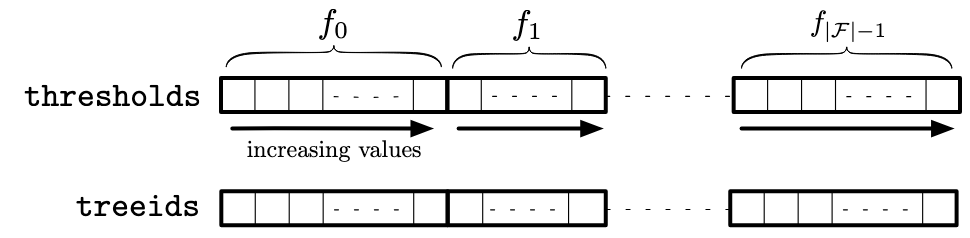
\includegraphics[width=0.8\textwidth]{img/QuickScorer2.png}
    \caption{Data structures used to store the thresholds and the tree IDs.}
\end{figure}